\documentclass[11pt,a4paper]{article}

% French
\usepackage[utf8x]{inputenc}
\usepackage[frenchb]{babel}
\usepackage[T1]{fontenc}
\usepackage{lmodern}
\usepackage{ifthen}

% Color
% cfr http://en.wikibooks.org/wiki/LaTeX/Colors
\usepackage{color}
\usepackage[usenames,dvipsnames,svgnames,table]{xcolor}
\definecolor{dkgreen}{rgb}{0.25,0.7,0.35}
\definecolor{dkred}{rgb}{0.7,0,0}

% Floats and referencing
\newcommand{\sectionref}[1]{section~\ref{sec:#1}}
\newcommand{\annexeref}[1]{annexe~\ref{ann:#1}}
\newcommand{\figuref}[1]{figure~\ref{fig:#1}}
\newcommand{\tabref}[1]{table~\ref{tab:#1}}
\usepackage{xparse}
\NewDocumentEnvironment{myfig}{mm}
{\begin{figure}[!ht]\centering}
{\caption{#2}\label{fig:#1}\end{figure}}

% Listing
\usepackage{listings}
\lstset{
  numbers=left,
  numberstyle=\tiny\color{gray},
  basicstyle=\rm\small\ttfamily,
  keywordstyle=\bfseries\color{dkred},
  frame=single,
  commentstyle=\color{gray}=small,
  stringstyle=\color{dkgreen},
  %backgroundcolor=\color{gray!10},
  %tabsize=2,
  rulecolor=\color{black!30},
  %title=\lstname,
  breaklines=true,
  framextopmargin=2pt,
  framexbottommargin=2pt,
  extendedchars=true,
  inputencoding=utf8x
}

\newcommand{\matlab}{\textsc{Matlab}}
\newcommand{\octave}{\textsc{GNU/Octave}}
\newcommand{\qtoctave}{\textsc{QtOctave}}
\newcommand{\oz}{\textsc{Oz}}
\newcommand{\java}{\textsc{Java}}
\newcommand{\clang}{\textsc{C}}
\newcommand{\keyword}{mot clef}

% Math symbols
\usepackage{amsmath}
\usepackage{amssymb}
\usepackage{amsthm}
\DeclareMathOperator*{\argmin}{arg\,min}
\DeclareMathOperator*{\argmax}{arg\,max}

% Sets
\newcommand{\Z}{\mathbb{Z}}
\newcommand{\R}{\mathbb{R}}
\newcommand{\Rn}{\R^n}
\newcommand{\Rnn}{\R^{n \times n}}
\newcommand{\C}{\mathbb{C}}
\newcommand{\K}{\mathbb{K}}
\newcommand{\Kn}{\K^n}
\newcommand{\Knn}{\K^{n \times n}}

% Chemistry
\newcommand{\std}{\ensuremath{^{\circ}}}
\newcommand\ph{\ensuremath{\mathrm{pH}}}

% Theorem and definitions
\theoremstyle{definition}
\newtheorem{mydef}{Définition}
\newtheorem{mynota}[mydef]{Notation}
\newtheorem{myprop}[mydef]{Propriétés}
\newtheorem{myrem}[mydef]{Remarque}
\newtheorem{myform}[mydef]{Formules}
\newtheorem{mycorr}[mydef]{Corrolaire}
\newtheorem{mytheo}[mydef]{Théorème}
\newtheorem{mylem}[mydef]{Lemme}
\newtheorem{myexem}[mydef]{Exemple}
\newtheorem{myineg}[mydef]{Inégalité}

% Unit vectors
\usepackage{esint}
\usepackage{esvect}
\newcommand{\kmath}{k}
\newcommand{\xunit}{\hat{\imath}}
\newcommand{\yunit}{\hat{\jmath}}
\newcommand{\zunit}{\hat{\kmath}}

% rot & div & grad & lap
\DeclareMathOperator{\newdiv}{div}
\newcommand{\divn}[1]{\nabla \cdot #1}
\newcommand{\rotn}[1]{\nabla \times #1}
\newcommand{\grad}[1]{\nabla #1}
\newcommand{\gradn}[1]{\nabla #1}
\newcommand{\lap}[1]{\nabla^2 #1}


% Elec
\newcommand{\B}{\vec B}
\newcommand{\E}{\vec E}
\newcommand{\EMF}{\mathcal{E}}
\newcommand{\perm}{\varepsilon} % permittivity

\newcommand{\bigoh}{\mathcal{O}}
\newcommand\eqdef{\triangleq}

\DeclareMathOperator{\newdiff}{d} % use \dif instead
\newcommand{\dif}{\newdiff\!}
\newcommand{\fpart}[2]{\frac{\partial #1}{\partial #2}}
\newcommand{\ffpart}[2]{\frac{\partial^2 #1}{\partial #2^2}}
\newcommand{\fdpart}[3]{\frac{\partial^2 #1}{\partial #2\partial #3}}
\newcommand{\fdif}[2]{\frac{\dif #1}{\dif #2}}
\newcommand{\ffdif}[2]{\frac{\dif^2 #1}{\dif #2^2}}
\newcommand{\constant}{\ensuremath{\mathrm{cst}}}

% Numbers and units
\usepackage[squaren, Gray]{SIunits}
\usepackage{sistyle}
\usepackage[autolanguage]{numprint}
%\usepackage{numprint}
\newcommand\si[2]{\numprint[#2]{#1}}
\newcommand\np[1]{\numprint{#1}}

\newcommand\strong[1]{\textbf{#1}}
\newcommand{\annexe}{\part{Annexes}\appendix}

% Bibliography
\newcommand{\biblio}{\bibliographystyle{plain}\bibliography{biblio}}

\usepackage{fullpage}
% le `[e ]' rend le premier argument (#1) optionnel
% avec comme valeur par défaut `e `
\newcommand{\hypertitle}[7][e ]{
\usepackage{hyperref}
{\renewcommand{\and}{\unskip, }
\hypersetup{pdfauthor={#6},
            pdftitle={Synth\`ese d#1#2 Q#3 - L#4#5},
            pdfsubject={#2}}
}

\title{Synth\`ese d#1#2 Q#3 - L#4#5}
\author{#6}

\begin{document}

\ifthenelse{\isundefined{\skiptitlepage}}{
\begin{titlepage}
\maketitle

 \paragraph{Informations importantes}
   Ce document est grandement inspiré de l'excellent cours
   donné par #7 à l'EPL (École Polytechnique de Louvain),
   faculté de l'UCL (Université Catholique de Louvain).
   Il est écrit par les auteurs susnommés avec l'aide de tous
   les autres étudiants, la vôtre est donc la bienvenue.
   Il y a toujours moyen de l'améliorer, surtout si le cours
   change car la synthèse doit alors être modifiée en conséquence.
   On peut retrouver le code source à l'adresse suivante
   \begin{center}
     \url{https://github.com/Gp2mv3/Syntheses}.
   \end{center}
   On y trouve aussi le contenu du \texttt{README} qui contient de plus
   amples informations, vous êtes invité à le lire.

   Il y est indiqué que les questions, signalements d'erreurs,
   suggestions d'améliorations ou quelque discussion que ce soit
   relative au projet
   sont à spécifier de préférence à l'adresse suivante
   \begin{center}
     \url{https://github.com/Gp2mv3/Syntheses/issues}.
   \end{center}
   Ça permet à tout le monde de les voir, les commenter et agir
   en conséquence.
   Vous êtes d'ailleurs invité à participer aux discussions.

   Vous trouverez aussi des informations dans le wiki
   \begin{center}
     \url{https://github.com/Gp2mv3/Syntheses/wiki}.
   \end{center}
   comme le statut des synthèses pour chaque cours
   \begin{center}
     \url{https://github.com/Gp2mv3/Syntheses/wiki/Status}.
   \end{center}
   vous pouvez d'ailleurs remarquer qu'il en manque encore beaucoup,
   votre aide est la bienvenue.

   Pour contribuer au bug tracker et au wiki, il vous suffira de
   créer un compte sur Github.
   Pour interagir avec le code des synthèses,
   il vous faudra installer \LaTeX.
   Pour interagir directement avec le code sur Github,
   vous devez utiliser \texttt{git}.
   Si cela pose problème,
   nous sommes évidemment ouverts à des contributeurs envoyant leurs
   changements par mail ou n'importe quel autre moyen.
\end{titlepage}
}{}

\ifthenelse{\isundefined{\skiptableofcontents}}{
\tableofcontents
}{}
}


\usepackage{graphicx}
\usepackage{caption}
\usepackage{subcaption}

\newcommand{\sbt}{\,\begin{picture}(-1,1)(-1,-3)\circle*{2.5}\end{picture}\ }
\newcommand{\umin}{u_\mathrm{min}}
\newcommand{\umax}{u_\mathrm{max}}

\usepackage{tikz}
\usepackage{pgfplots}
\usetikzlibrary{arrows,calc}

\hypertitle{Automatique Linéaire}{6}{INMA}{1510}
{Benoît Legat}
{Denis Dochain}

% http://me.berkeley.edu/~maxchen/_static/block_diagram_in_latex.pdf
\tikzstyle{block} = [draw, rectangle, minimum height=2em, minimum width=4em]
%fill=blue!20
\tikzstyle{sum} = [draw, fill=blue!20, circle, node distance=1cm]
\tikzstyle{input} = [coordinate] \tikzstyle{output} = [coordinate]
\tikzstyle{pinstyle} = [pin edge={to-,thin,black}]

\section{Règle de Mason}
Le principe est expliqué assez clairement dans \cite{chau2002mason}
avec des exemples pour illustrer.
En résumé, on considère le schéma bloc comme un graphe dirigé et
pour calculer la fonction de transfert entre $a$ et $b$.
On prend
\begin{itemize}
  \item tous les chaines directes $F_k$ (c'est des chemins pour prendre la vocable des graphes, ce qui signifie qu'on ne fait pas de cycle),
  \item toutes les boucles $\{L_i\}$ (les cycles dans le vocable des graphes),
  \item toutes les boucles qui ne touchent \emph{pas} $F_k$: $\{L_{k;i}\}$.
\end{itemize}
Et on a la fonction de transfert par la formule suivante
\[ H(s) = \frac{\sum_k F_k\Delta(\{L_{k;i}\})}{\Delta(\{L_i\})} \]
où
\[ \Delta(\{L_j\}) = 1 - \sum_{j_1} L_{j_1} + \sum_{j_1,j_2} L_{j_1}L_{j_2} - \sum_{j_1,j_2,j_3} L_{j_1}L_{j_2}L_{j_3} + \cdots \]
avec $j_1, j_2, \ldots, j_n$ tels que les boucles $L_{j_1}, L_{j_2}, \ldots, L_{j_n}$ ne se touchent \emph{pas}.
Si toutes les boucles, se touchent, ça devient donc simplement
\( 1 - \sum_{j_1} L_{j_1}. \)
On remarque que $\Delta(\emptyset) = 1$.
La plupart du temps, les chaines directes touchent toutes les boucles et le numérateur devient donc $\sum_k F_k$ car $\{F_{k;i}\} = \emptyset$.

\begin{myexem}
  \label{ex:masonex}
  Pour l'exemple de la \figuref{masonex}, on a
  \begin{itemize}
    \item deux chaines directes qui valent respectivement $A(s)C(s)$ et $A(s)D(s)$,
    \item deux boucles qui valent respectivement $-A(s)B(s)$ et $D(s)E(s)$,
    \item la première chaine directe ne touche que par la première boucle et la deuxième passe les touchent toutes.
  \end{itemize}
  On a donc, comme les deux boucles ne se touchent pas,
  \[ H(s) = \frac{A(s)C(s)(1 - D(s)E(s)) + A(s)D(s)}{1 + A(s)B(s) - D(s)E(s) - A(s)B(s)D(s)E(s)}. \]
  \begin{figure}[!ht]
    \centering
    \begin{tikzpicture}[auto, node distance=2cm,>=latex']
      \node [input, name=input] {};
      \node [sum, right of=input] (sum) {};
      \node [block, right of=sum, node distance=2cm] (A) {$A(s)$};
      \node [block, below of=A] (B) {$B(s)$};
      \node [block, right of=A, node distance=6cm] (C) {$C(s)$};
      \node [block, below of=C, node distance=2cm] (D) {$D(s)$};
      \node [block, below of=D, node distance=2cm] (E) {$E(s)$};
      \node [sum, right of=C, node distance=2cm] (sum2) {};
      \node [sum, left of=D, node distance=1.5cm] (sum3) {};
      \node [output, right of=sum2] (output) {};
      \draw [->] (input) -- node {$a(t)$} (sum);
      \draw [->] (A) -- node[name=Ar,pos=0.3] {} node[name=Cl,pos=0.7] {} (C);
      \draw [->] (Ar) |- (B);
      \draw [->] (B) -| node[pos=0.45] (Bl) {} node[pos=0.95] {$-$} (sum);
      \draw [->] (sum) -- (A);
      \draw [->] (Cl) |- (sum3);
      \draw [->] (sum3) -- (D);
      \draw [->] (C) -- (sum2);
      \draw [->] (D) -| node[pos=0.3] (Dr) {} (sum2);
      \draw [->] (Dr) |- (E);
      \draw [->] (E) -| (sum3);
      \draw [->] (sum2) -- node {$b(t)$} (output);
    \end{tikzpicture}
    \caption{Schéma-block de l'exemple~\ref{ex:masonex}.}
    \label{fig:masonex}
  \end{figure}
\end{myexem}

\section{Emballement}

\begin{figure}[!ht]
  \centering
  \begin{tikzpicture}[auto, node distance=2cm,>=latex']
    \node [input, name=input] {};
    \node [sum, right of=input] (sum) {};
    \node [block, right of=sum, node distance=2cm] (C) {$k_p + \frac{k_i}{s}$};
    \node [block, right of=C, node distance=4cm] (S) {$\max(\umin,\min(\umax,\sbt))$};
    \node [block, right of=S, node distance=4cm] (G) {$G(s)$};
    \node [sum, right of=G, node distance=2cm] (sum2) {};
    \node [block, above of=sum2, node distance=1.5cm] (H) {$H(s)$};
    \node [input, above of=H, name=pert, node distance=1cm] {};
    \node [output, right of=sum2] (output) {};
    \node [below of=S] (feedback) {};
    \draw [->] (input) -- node {$r(t)$} (sum);
    \draw [->] (pert) -- node {$v(t)$} (H);
    \draw [->] (H) -- (sum2);
    \draw [->] (C) -- node {$u_c(t)$} (S);
    \draw [->] (S) -- node {$u(t)$} (G);
    \draw [->] (sum) -- node {$e(t)$} (C);
    \draw [->] (G) -- (sum2);
    \draw [->] (sum2) -- node[name=y] {$y(t)$} (output);
    \draw (y) |- ($(S)+(0,-1.5cm)$);
    \draw [->] ($(S)+(0,-1.5cm)$) -| node[pos=0.95] {$-$} (sum);
  \end{tikzpicture}
  \caption{Schéma-block d'un système avec saturation.}
  \label{fig:windup-block}
\end{figure}

Toute notre analyse se base sur le fait que nous avons des systèmse LTI (Linear Time Invariant).
Pourtant, en pratique, il y a pas mal de cause de non-linéaire.
Une assez courante est la \emph{saturation} de la commande.
Ça a lieu lorsque le système ne sait qu'appliquer une commande entre $\umin$ et $\umax$.
On modélise alors notre système avec une composante non-linéaire appelée saturation.
Son entrée est la commande voulue $u_c$ et sa sortie la commande vraiment appliquée $u$.
On a la relation $u = \min(\umax, \max(\umin, u_c))$, c'est à dire que si $u_c \geq \umax$,
on prend $u = \umax$ et si $u_c \leq \umin$, on prend $u = \umin$, sinon on a $u = u_c$.
Le système est représenté par la \figuref{windup-block}.

Comme la composante de saturation est non-linéaire on ne peut plus représenter cette composante
par une convolution en temporelle ou un produit en fréquentiel et on ne peut donc faire d'analyse
fréquentielle.

\begin{figure}
  \centering
  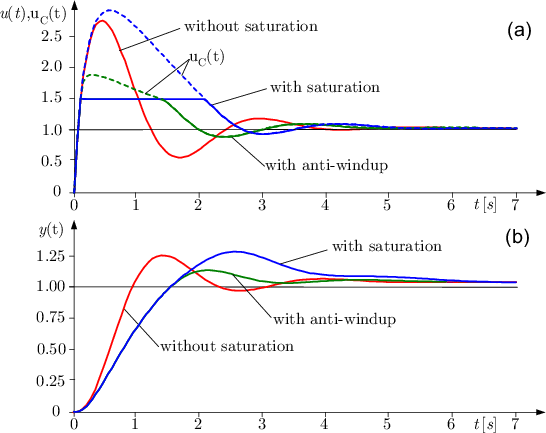
\includegraphics[width=0.6\linewidth]{schmidwindup.png}
  \caption{Exemple de l'application d'un système anti-emballement pris de~\cite{schmid2005windup}.
  La courbe rouge montre le comportement du système sans saturation.
  On rajoute une saturation à \num{1.5} pour la courbe bleue.
  La courbe verte a la saturation et le système emballement.}
  \label{fig:schmidwindup}
\end{figure}

Dans la \figuref{schmidwindup}, on voit que sans la saturation,
on arrive plus vite à la consigne.
Avec la saturation, $u$ n'est pas aussi grand qu'on aimerait et on va donc
moins vite.
Cette lenteur fait que l'intégrale a plus le temps de gonfler.
En effet, on voit que l'aire entre la consigne 1 et la courbe rouge dans
le graphe de $y$ est plus petite que celle entre la consigne et la courbe bleue.
Lorsqu'on atteint la consigne, l'intégrale est donc plus grosse pour le système
avec saturation.
Il va donc prendre beaucoup plus de temps à réaliser qu'il faut redescendre
et l'intégrale risque d'à nouveau trop gonfler.

\begin{figure}
  \centering
  \begin{subfigure}{0.49\linewidth}
    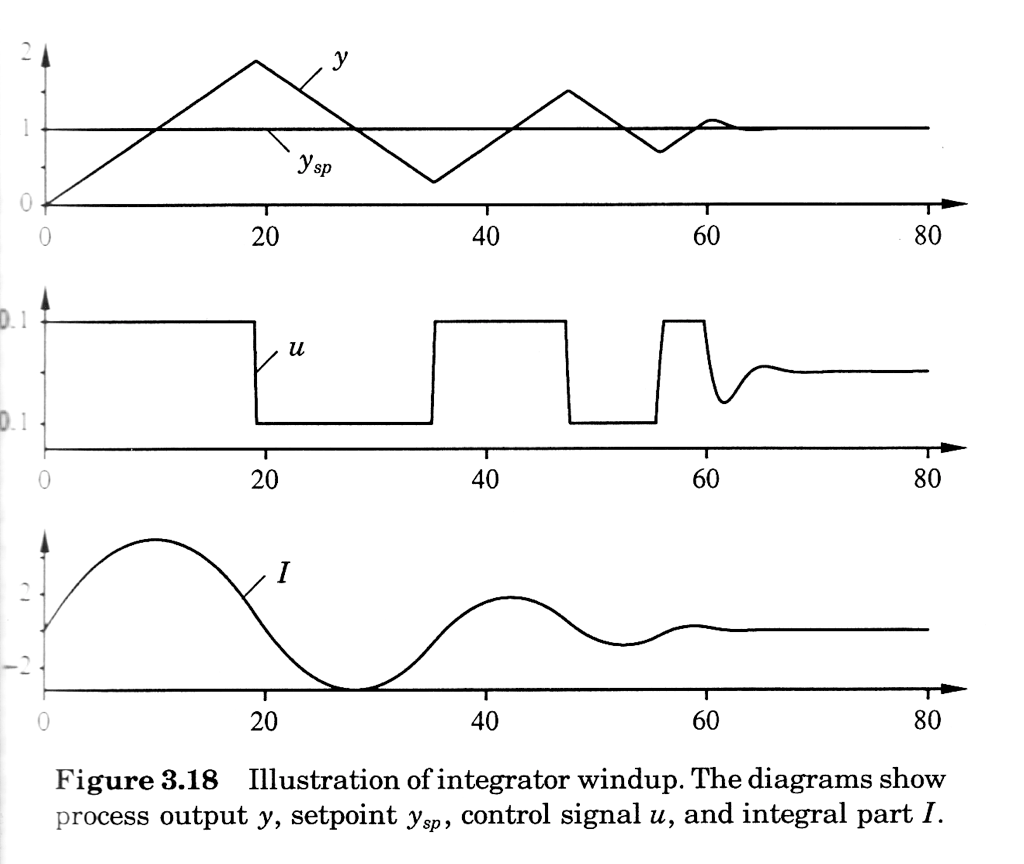
\includegraphics[width=\linewidth]{windup.png}
    \caption{Exemple d'emballement.}
    \label{fig:windup}
  \end{subfigure}
  \begin{subfigure}{0.49\linewidth}
    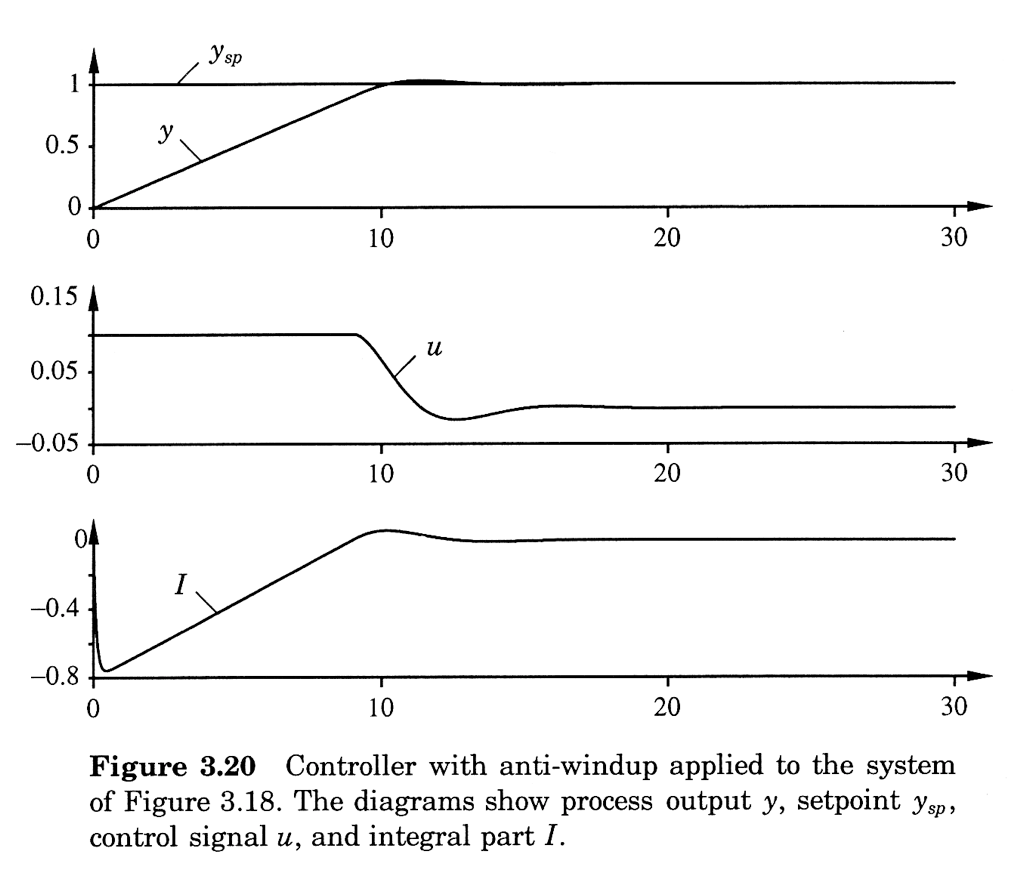
\includegraphics[width=\linewidth]{anti-windup.png}
    \caption{Application d'un système anti-emballement à l'exemple de la \figuref{windup}.}
    \label{fig:anti-windup}
  \end{subfigure}
  \caption{Exemple d'emballement avec application d'un système anti-emballement.}
  \label{fig:windup-cm}
\end{figure}

Il arrive qu'il prenne tellement de temps à s'en rendre compte, c'est à dire
que l'intégrale prend tellement de temps à dégonfler que l'erreur est très
grande lorsque l'intégrale est enfin nulle se qui fait qu'on atteint l'autre borne
pour de la commande très rapidement.
On est alors reparti pour un tour.
C'est ce qu'on observe à la \figuref{windup} en $t = 19$,
dans le graphe de $u$, on passe tellement vite d'une borne à l'autre qu'on a l'impression
que c'est un point de discontinuité.
On voit en effet, en regardant le graphe pour $y$ à $t = 19$ qu'on avait atteint une erreur
assez importante.

\subsection{Système anti-emballement}

\begin{figure}[!ht]
  \centering
  \begin{tikzpicture}[auto, node distance=2cm,>=latex']
    \node [input, name=input] {};
    \node [sum, right of=input] (sum) {};
    \node [sum, right of=sum] (sum4) {};
    \node [block, right of=sum4, node distance=2cm] (C) {$k_p + \frac{k_i}{s}$};
    \node [block, right of=C, node distance=4cm] (S) {$\max(\umin,\min(\umax,\sbt))$};
    \node [block, right of=S, node distance=4cm] (G) {$G(s)$};
    \node [sum, right of=G, node distance=2cm] (sum2) {};
    \node [block, above of=sum2, node distance=1.5cm] (H) {$H(s)$};
    \node [input, above of=H, name=pert, node distance=1cm] {};
    \node [output, right of=sum2] (output) {};
    \node [below of=S] (feedback) {};
    \draw [->] (input) -- node {$r(t)$} (sum);
    \draw [->] (pert) -- node {$v(t)$} (H);
    \draw [->] (H) -- (sum2);
    \draw [->] (C) -- node[below,name=uc] {$u_c(t)$} (S);
    \draw [->] (S) -- node[below,name=u] {$u(t)$} (G);
    \draw [->] (sum) -- node {$e(t)$} (sum4);
    \draw [->] (sum4) -- (C);
    \draw [->] (G) -- (sum2);
    \draw [->] (sum2) -- node[name=y] {$y(t)$} (output);
    \draw (y) |- ($(S)+(0,-1.5cm)$);
    \draw [->] ($(S)+(0,-1.5cm)$) -| node[pos=0.95] {$-$} (sum);

    \node [block, above of=C, node distance=1.5cm] (a) {$\alpha$};
    \node [sum, above of=uc, node distance=1.85cm] (sum3) {};
    \draw [->] (sum3) -- (a);
    \draw [->] (uc) -- node[pos=0.9] {$-$} (sum3);
    \draw [->] (u) |- (sum3);
    \draw [->] (a) -| (sum4);
  \end{tikzpicture}
  \caption{Schéma-block d'un système avec saturation et système anti-emballement.}
  \label{fig:anti-windup-block}
\end{figure}

On voit que les problèmes d'emballement sont liés à la composantes intégrale.
Il nous faut alors, pour remédier à l'emballement, ajouter un système qui détectera quand
$u_c \geq u$, c'est à dire que $u_c \geq \umax$ ou $u_c \leq u$, c'est à dire $u_c \leq \umin$,
et qui videra l'intégrale qui est trop positive ou trop négative.
Un système anti-emballement classique est représenté par la \figuref{anti-windup-block}.

\begin{itemize}
  \item Si $u = u_c$, ce système n'a aucun effet car $u - u_c = 0$.
  \item Si $u \leq u_c$, ça peut signifier 2 choses
    \begin{description}
      \item[Une trop grosse action proportionnelle]
        L'erreur est très grande par rapport à $\umax$, ou plus précisément que $k_p e(t) \gg \umax$,
        on va donc être trop lent pour arriver à $e(t) = 0$ et on va donc intégrer plus que voulu.
        $u - u_c$ est négatif, avec $e + \alpha (u-u_c)$ comme entrée à $C(s)$,
        on aura toujours $\umax \leq u_c$\footnote{même si $\alpha$ est grand, on ne peut pas avoir $u_c < \umax$ car alors $u = u_c$ et on et donc il n'y a plus que $e$ à l'entrée de $C(s)$ et donc $\umax \leq u_c$.}
        mais on intégrera $e + \alpha (u-u_c) < e$, même si on intégrera plus longtemps que sans la saturation, on intégrera moins,
        l'intégrale sera alors moins gonflée lorsqu'on aura $e(t) = 0$.
      \item[Une trop grosse action intégrale]
        L'erreur n'est plus spécialement grande, elle est même peut-être déjà devenue négative mais
        on continue à vouloir $u_c \geq \umax$ à cause de l'intégrale qui a beaucoup gonflé.
        Pour la même raison que précédemment, on aura toujours $u_c \geq \umax$,
        l'effet va être donc uniquement dans l'intégrale, on va la vider plus rapidement qu'elle se viderait normalement.
    \end{description}
  \item Si $u \geq u_c$, la discussion est pareille que pour $u \leq u_c$.
\end{itemize}
En résumé, l'action du système va être sur l'intégrale, elle va l'empêcher de trop gonfler et puis va la vider plus rapidement.
Elle ne va cependant agir que lorsque la commande sature et ne va donc pas poser de problème dans les cas où il n'y a pas de risque
d'emballement.
Elle ne va faire \emph{pas} descendre $u_c$ en dessous de $\umax$ ou au dessus de $\umin$ quand on sature,
elle ne va donc \emph{pas} augmenter le temps de réponse.

Illustrons cela avec pour commencer la \figuref{schmidwindup} où on voit que le seul effet du système anti-emballement est lorsqu'on dépasse
$\umax = 1.5$.
On voit en pointillé $u_c$ qui est plus petit que pour a courbe bleue mais qui ne descend pas en dessous de $\umax$ tant que $y(t) \leq r(t)$.
Il est par contre beaucoup plus rapide à passer en dessous de $\umax$ lorsuqe $y(t) \geq r(t)$ ce qui montre bien qu'il a empêché à l'intégrale de trop gonfler.

Pour la \figuref{anti-windup}, on voit à nouveau que le système anti-emballement ne fait pas passer $u_c$ en dessous de $\umax$.
Au tout début, on voit que l'intégrale intégre quelque chose de très négatif, ça doit être dû au fait qu'au début, on demande un
très grand $u_c$ et donc $\alpha (u_c-u)$ est très négatif.
Par la suite, comme $\alpha(u_c-u)$ est négatif, l'action proportionnelle est moins forte et l'action intégrale est négative donc
$u_c - u$ est moins important, de telle sorte que $e(t) \geq -\alpha (u_c - u)$, on intègre donc du positif et l'intégrale remonte.
Elle monte d'ailleurs beaucoup plus lentement que pour la \figuref{windup} grâce au fait qu'on intègre aussi $\alpha (u_c - u)$ qui
est négatif.
Au final, lors $y(t) \geq r(t)$, l'intégrale est vide et $u$ ne sature plus, on repasse donc dans un système LTI et le système
anti-emballement n'a plus d'effet.

% TODO astrom p. 307pdf 295vrai

\biblio

\end{document}
